\documentclass[10pt,dvips]{article}
\usepackage{epsfig}
\usepackage{fancyheadings}
%\usepackage{twocolumn}
\usepackage{verbatim,moreverb,doublespace}
%\usepackage{rotate,lscape,dcolumn,array,rotating,latexsym}

\topmargin=-0.6in
\setlength{\oddsidemargin}{0.0 in}
\setlength{\textheight}{9.0in}
\setlength{\textwidth}{6.5in}
%\renewcommand{\thepage}{2}
\renewcommand{\baselinestretch}{1.0}
\renewcommand{\thesection}{\Roman{section}}
\renewcommand{\thesubsection}{\Alph{subsection}}
\renewcommand{\thesubsubsection}{\Alph{subsection}.\arabic{subsubsection}}


\pagestyle{fancy}
\lhead{}
\chead{\bf University of Rhode Island - CONFIDENTIAL}
\rhead{}
\lfoot{}
\cfoot{\thepage}
\rfoot{}


\begin{document}

\begin{center}
{\Large \bf University of Rhode Island}\\
{\Large \bf Invention Disclosure Statement}\\
\vspace{0.1in}
Augustus K. Uht - URI\\
David Morano - Northeastern University\\
David Kaeli - Northeastern University\\
January 11, 2000
\end{center}

\section{Description}
%\setcounter{subsection}{1}
\subsection{Invention Title}
{\bf ``Resource Flow Computer''}


\subsection{Description}
\label{desc}
This invention will increase the performance of traditional processors through the
use of highly speculative code execution. The technique may be used with any
instruction set, including the Intel x86 or IA-32 instruction set. The invention
uses substantially less hardware than prior methods and the hardware is also less
complex.

One other extremely important characteristic of the invention is that it is
the first ILP (Instruction Level Parallelism) or superscalar processor using
hardware to enforce correct program execution that is {\it scalable}. By the term
``scalable'' we mean that the hardware cost (number of transistors) grows
\underline{linearly} with the number of execution units in the machine.

The mechanisms give rise to the machine's scalability also result in the machine
having relatively constant critical path delay with respect to an increase in the
number of execution units. This happens because much of the computation of the
machine is localized to small regions of the machine.


\subsubsection{Background}
\label{background}
Traditionally, computers have used a {\it control flow} model of program execution.
This model is an imperative model: the user tells the computer which instructions to
execute and when. Instructions may be conditionally executed or repeatedly
executed with the use of {\it branches} at the machine level. A branch causes
the computer to (conditionally) change the order in which instructions are
to be executed. In the traditional model instructions are executed one at a time,
strictly in the specified order.

In recent years computer designers have sought to improve performance by
executing more than one instruction at a time and possibly out-of-order. This is
an exploitation of {\it Instruction Level Parallelism (ILP)}, also popularly known
as a ``superscalar'' approach. ILP is possible because not all instructions' inputs
come from immediately-prior instructions.

Ignoring control flow for the minute, the
only necessary constraint to ensure correct program execution is to generate instruction
results before they are supposed to be used by other instructions. Thus, say an
instruction {\tt x = y + z} is waiting to execute; as soon as both of its inputs
{\tt y} and {\tt z} have been generated the instruction may execute or {\it fire},
sending inputs to an adder, the adder performing the operation and then saving
the result in variable or register {\tt x}. Instructions waiting for the new value
of {\tt x}, that is having {\tt x} as an input, may then potentially fire themselves.
This is a case of the waiting instruction being {\it data dependent} on the former.
This type of execution model is called the {\it data flow} model.

Modern processors present the appearance of the traditional control flow model to
the user, but employ a data flow model ``under the hood''. Thus, the relative
conceptual
simplicity of the control flow model is maintained with the improved performance of
the data flow model.

In the data flow model branches must still be used and are problematic. The typical
approach today is to {\it predict} the outcome of conditional branches and then
{\it speculatively} execute the corresponding code. Once the value of the
branch condition is known, the branch is said to have {\it resolved}. If the
prediction was correct, nothing special need be done. If there was a
{\it misprediction}, however, the computer must effectively reset its state to
what it was just before the branch was first encountered. Even though
branch predication accuracies for real code are at or above 90\%, mispredictions
are still a great impediment to obtaining higher performance.

In prior work\cite{Uht95} we demonstrated a variation of branch speculation called
{\it Disjoint Eager Execution (DEE)} which may vastly improve computer performance.
DEE is a form of {\it multipath} execution; code is executed down both paths from
a branch. The code execution is unbalanced; code on the predicted path is given
preferential priority for execution resources over code on the not-predicted path.
When the branch resolves, results for either branch direction are available,
and hence the performance penalty due to a misprediction is greatly reduced.
ILP of the order of ten's of instructions executing at once was shown to be
possible, as compared with an ILP of 2-3 instructions in existing processors.

Our prior proposed machine realization of DEE with a data flow equivalent
required many large
and cumbersome data dependency and control dependency bit matrices. Data and control
issues were treated separately. Approaches to reducing the size of the
matrices were partially devised but never proven.

Other approaches, including current microprocessors, also need a lot of hardware to
realize data flow even with simple branch prediction. In particular, data dependencies
must still be computed and other complex operations performed for code to be correctly
executed. Hence all of these other ILP approaches are not scalable in that
their hardware cost typically grows as the square of the number of execution units in
the machine.

Other researchers have demonstrated the value of {\it data speculation}
\cite{Lipasti96,Sazeides96}.
In this scenario, input values for some instructions are predicted and the
instructions allowed to execute speculatively. As with control speculation,
there is a penalty for data value misprediction.
No one has yet, to our knowledge, combined data speculation with DEE.

\subsubsection{The Subject Invention}
The basic model of execution of the subject invention is radically different
from what has come before. The new model is the {\it resource flow} or
{\it squash flow} execution model. There are a few key concepts of
this model that describe its operation and characteristics:
\begin{enumerate}
\item As with most processors, candidate instructions for execution are loaded from
memory into an {\it instruction window}. This is high-speed storage present in the
processor itself. When instructions fire they are sent with their data inputs to
Processing Elements (execution units such as adders, etc.) for execution.

\item Unlike most processors, the invention has associated with each candidate
instruction a {\it time tag} indicating the instruction's nominal sequential order
in the program being executed.

\item The basic resources of the computer, the {\it Processing Elements (PE)}
containing the adders, multipliers and logic functions, always execute the
instructions with the highest priority. The PE's always look for work, hence
the ``resource flow'' terminology; this could also be called ``resource-driven''.

\item Instructions execute regardless of their data or control dependencies.
Instructions execute or re-execute only when one or more of their inputs has changed
value; thus when an input changes value the instruction effectively {\it squashes}
or nullifies its current result and generates a new, updated value for the result.

\item Newly-generated results are broadcast to all of the instructions in the
window, along with the results' identifying address and time tag.

\item Instructions in the window look at or ``snoop'' the broadcast information,
copying or ``snarfing'' matching results for their input(s). If there is a match,
and the broadcast value differs from the current value of the input,
such instructions fire and the process repeats.
\end{enumerate}

Other important ideas are:
\begin{enumerate}
\item Full hidden-explicit predication is used to realize control flow (see
companion invention disclosure by the same authors).

\item Every instruction has predicate inputs and outputs. The inputs tell the
instruction when its result should modify the state of the machine (classically,
this is equivalent to indicating whether or not an instruction should execute).
The outputs are fed to other instructions. The major predicate outputs are those
from branches.

\item Predicate inputs and outputs are treated the same as instruction data
inputs and outputs: predicate (and data) instruction outputs
are recomputed only if a predicate input (or data input) changes value; the
newly-generated results are broadcast with their address and time identifiers
to all of the instructions in the window.
\end{enumerate}

\subsubsection{Detailed Description - Preferred Embodiment}
The following sections give detailed descriptions of the processor components that
are either novel parts of the invention or traditional components
necessary for the invention's operation. Novel parts are marked as such.

\paragraph{High-Level Microarchitecture: }
Instructions in the resource flow computer are combined into novel {\it sharing groups}
in order to
share certain machine resources, including PE's; see Figure~\ref{sharinggroups}.
Only one instruction in a group may fire in a given clock cycle and supply source data
to the group's PE. The output of the PE goes back to the corresponding instruction,
as well as being broadcast to groups later in the nominal temporal sequential order.

\begin{figure}
\centering
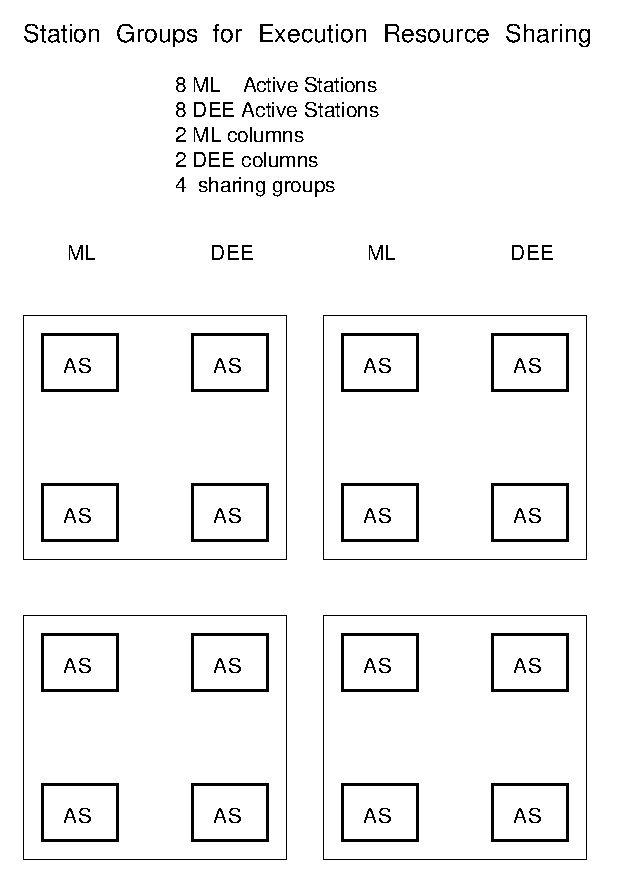
\epsfig{file=sharing.eps,width=3.50in}
\caption{{\em Sharing Groups.} Four sharing groups are shown, each having two ML
and two DEE active stations. Normally one PE is assigned to and services the
execution demands of one sharing group. `AS' stands for {\it Active Station}; each
AS holds one instruction.}
\label{sharinggroups}
\end{figure}

A block diagram of the high-level microarchitecture of the resource flow computer is
presented in Figure~\ref{highlevelma}. The memory system is designed so as to
satisfy the bandwidth requirements of the processor; it includes appropriately many
levels and sizes of caches and memory banks. The instruction fetch hardware is able
to supply the instruction bandwidth needed by the processor.

\begin{figure}
\centering
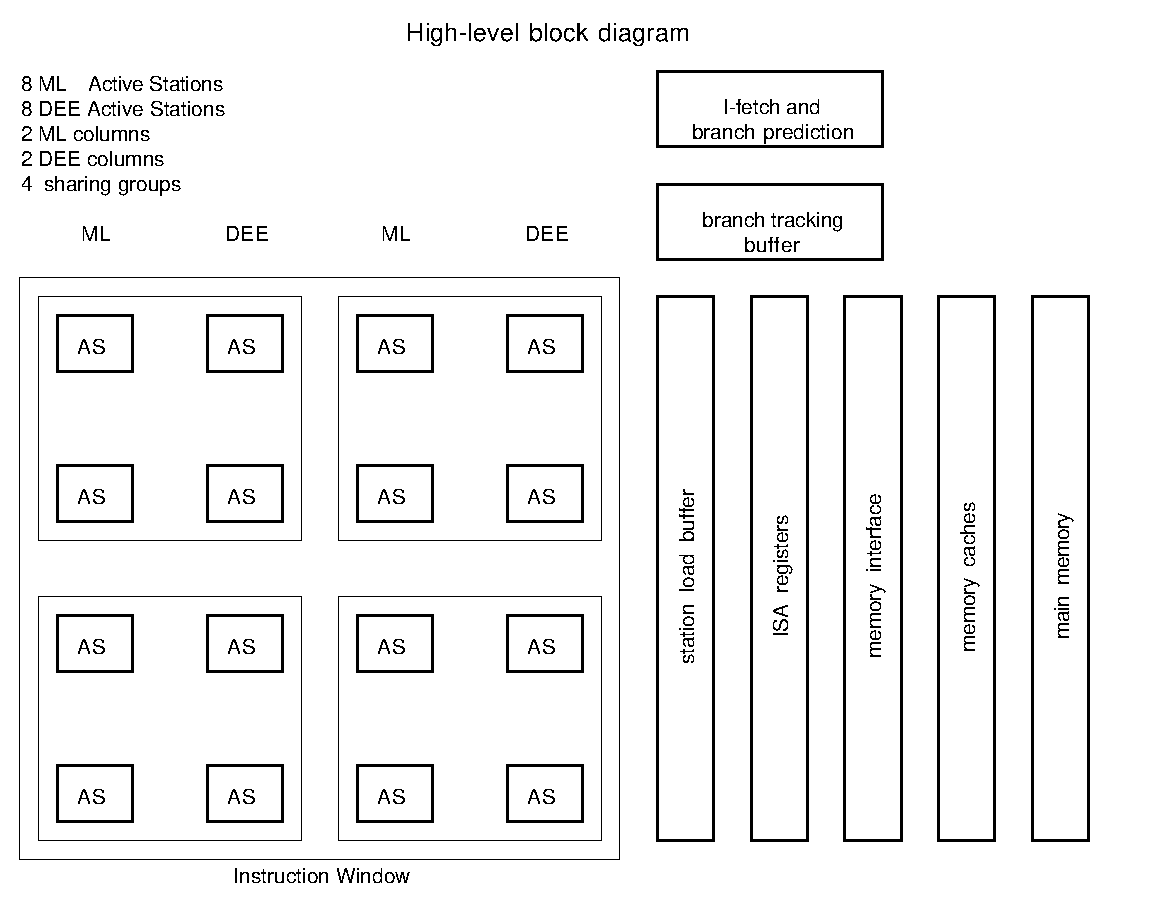
\epsfig{file=high.eps,width=6.50in}
\caption{{\em Resource flow computer high level microarchitecture.}
The primary differentiating component is the instruction window.}
\label{highlevelma}
\end{figure}

There are a large number of PE's available to execute
instructions. Each PE is able to execute any type of instruction in the instruction
set of the computer. As such they are very general devices. Although we will use this
PE model for discussion purposes in the following text, in a real machine the PE's
might be divided into multiple {\it functional units}, each one specialized for
one or more particular functions, e.g., floating point operations; this is standard
practice. Typically there might be 32 PE's in a resource flow computer.

The {\it instruction window} (this version is novel)
holds a subset of the instructions in the program
being executed in the {\it static order}. The static order is the order of
instructions as they have been written, or in other words the order as exists
in memory. This order is nominally independent of the actual dynamic execution
of the control flow (branches) and hence is relatively easier to generate than
a dynamically-ordered window. In practice, the order of the code in the window
is a combination of the static and dynamic orders. While we have proposed
static windows in our prior work\cite{Uht91,Uht92,Uht95}, no real machine,
or any other type of machine, for that matter, has used a static window.

In order to make the assignment of resources to instructions
easier and less expensive, the instruction window is {\it folded} as is shown in
Figure~\ref{foldediwindow} for a 4-by-4 window. All instructions on a single row
share one resource, such as a register file copy. Thus, each register file copy
serves every fourth instruction. 
Instructions corresponding to DEE paths are physically arranged as shown in
Figure~\ref{deeiwindow}.

\begin{figure}
\centering
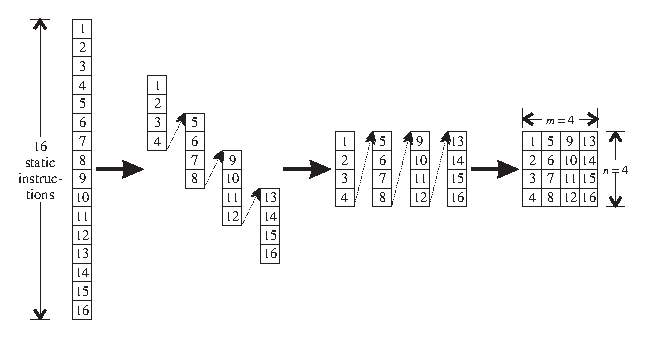
\epsfig{file=iw.eps,width=6.50in}
\caption{{\em Folding the Instruction Window.} An instruction window (IW) nominally 16
static instructions long is shown logically (on the left) and folded (on the right).
Each box represents an {\it active station}, ordered in time as indicated by the numbers,
larger numbers being later in time. An active station holds one instruction.}
\label{foldediwindow}
\end{figure}

\begin{figure}
\centering
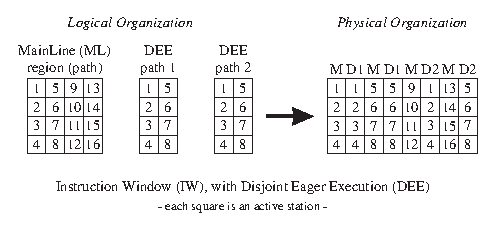
\epsfig{file=iwdee.eps,width=5.50in}
\caption{{\em Instruction Window with DEE.} The instruction window is shown with
the DEE paths incorporated (interlaced) with the ML path.}
\label{deeiwindow}
\end{figure}


The {\it load
buffer} is a staging area for fetching and holding instructions until the buffer is
filled and the instruction window is ready to accept a new buffer's worth of
instructions. Typically this involves
fetching a number of instructions equal to the number of instruction rows or
processing elements every
cycle. The fetched instructions are shifted from the fetch buffer into the
instruction window when the buffer is full and the first column of instructions in the
window, the earliest, have been fully executed (their results will not change).

The logical
ISA register file (ISAR) holds the current values of the registers present in the
Instruction Set Architecture of the computer, that is, the registers visible to
the user. The ISAR is constantly updated with values generated by the PE's; therefore,
the ISAR holds the latest-generated values of registers.
As part of instruction fetching the source values, or data inputs,
of each new instruction are initialized to the values held in the ISAR; this is novel.
Other types
of data speculation may be substituted or added to this basic method.

The ISAR is realized physically with multiple copies of the same ISAR file, see
Figure~\ref{isaregisters}. Each copy is associated with a single row of active
stations. A file is read when the rightmost column of active stations is
loaded from the load buffer. Reads from a file only go to the rightmost active
station on the same row. This approach increases the effective bandwidth
of the logical ISAR; the approach is common in the art, but is unique in its
application here. Writes to the ISAR may be made simultaneously from every
row of the instruction window; each copy is updated with the value of its
corresponding
write. Since all of the writes may be to the same register address and all of the
register file copies must contain the same data (must be {\it coherent}), a
novel scheme is used to resolve multiple writes to the same address; it is
described later in this document.

\begin{figure}
\centering
\epsfig{file=reg1.eps,width=4.50in}
\caption{{\em Microarchitecture of the ISA Register File.} The ISA register file is
replicated once for each row of the instruction window. All active stations in the
rightmost (later) column are loaded simultaneously, each station from the file
associated with its row. The files are triple-read ported, since an active station
may have two regular register sources and one relay register source (these are
described later).}
\label{isaregisters}
\end{figure}

The core of the machine (the instruction window) interfaces to
main memory through a special memory interface, shown in more
detail in Figure~\ref{memory}.  This memory interface filters memory
reads to see if they can be satisfied by outstanding memory
reads or writes to the same address.  Memory references to different
addresses may be out-of-order, unless they go to the Input/Output
section of the computer. Memory reads and writes to the same address
are also filtered to maintain a correct program order of memory
references between homogeneous groups of reads and groups of writes.
References within either type of group may be out-of-order with
respect to the instruction
window. Write references to the same address are kept in-order with respect to
the memory itself. In some cases multiple writes to the same address can be
reduced to a single write. Further details of how this memory interface
functions is provided in the technical report entitled
"High Performance Memory System for High ILP Microarchitectures"
by Uht \cite{Uht97e}; it is not part of the novel material of this invention
(it is in the public domain).
This is the suggested memory system for the
resource flow computer,
designed to provide high bandwidth and low latency. Other memory
systems with similar attributes may be used with suitable modification.

\begin{figure}
\centering
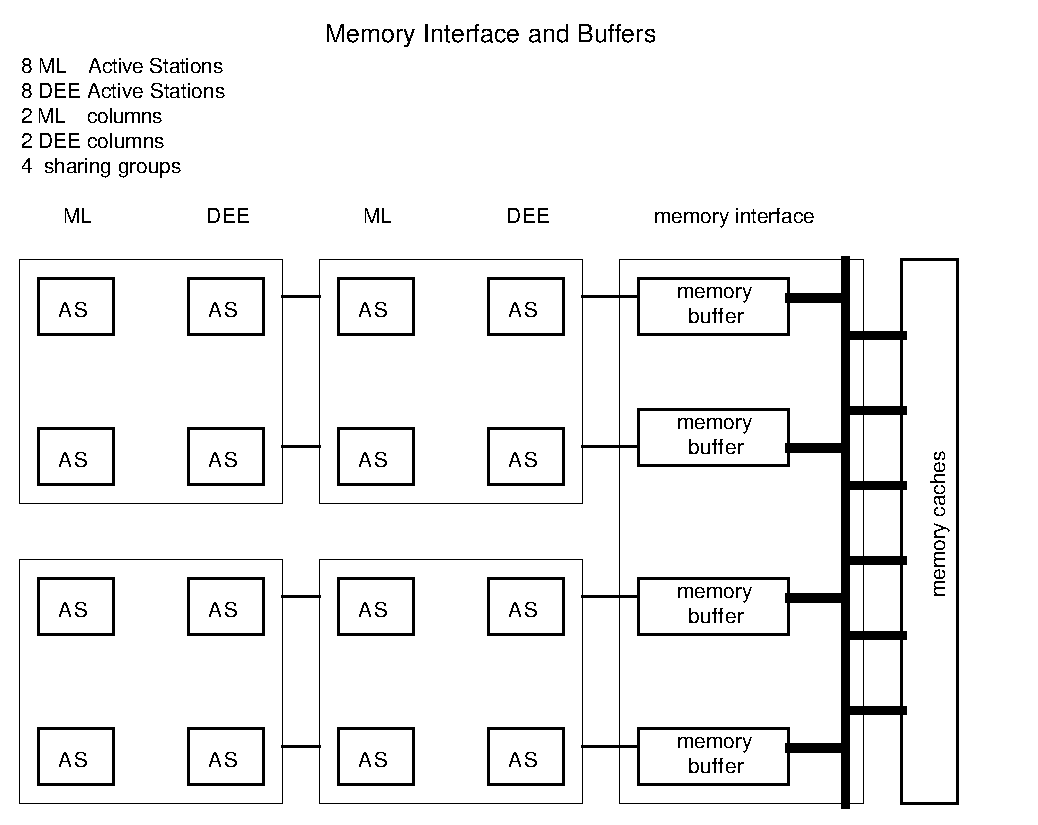
\epsfig{file=memory1.eps,width=5.50in}
\caption{{\em Memory system.} A suggested memory system for the resource flow
computer.}
\label{memory}
\end{figure}

The branch predictor predicts branches as they are encountered by the instruction
loader. A prediction is used to set the values of the predicates of instructions
loaded after the branch. These initial predicate values are loaded into the
instruction window with each instruction.

Every cycle the instruction in each sharing group
with the highest priority (earliest in
the order, with ML before DEE stations) that is ready to execute is issued to the
PE corresponding to the
instruction's sharing group.
Included with the issuing data are the address of the result and
the time tag of the instruction (same as the time tag of the result).
Once the PE has finished computing a value for an instruction, the value with
its address and time tag
is logically
broadcast to all instructions in the instruction window. As is described
later, the preferred embodiment does not actually broadcast all results
directly to every station.
According to three
conditions to be specified later, an instruction in the window may copy the
value into its storage. This method of data communication among
stations in the window using time tags is novel.

\paragraph{Instruction Window and Time Tags: }
Each instruction in the instruction window has associated with it a dynamically
changing  {\it time tag}. The time tag is formed as the concatenation of the
column address of the instruction with the row address of the instruction. This
composite tag is just the position of the instruction in the window.
In the following discussion, for the sake of simplicity we assume that
the time tags
are fixed with respect to the physical instruction cells. In reality, the columns
of cells can be renamed, i.e., any physical column can effectively be the ``leftmost''
column. While renaming in general is not novel, its use here is.

When every instruction in the leftmost or earliest column has finished executing,
the column is {\it retired} by effectively shifting the entire window contents
to the left by one column. This changes the time tags of every instruction in
the window, effectively decrementing the column address part of every instruction's
time tag by one. The automatic updating of the time tags throughout the window is
novel. The results from the retired column are sent to both the register
file copies and the memory system, as appropriate.

Each instruction cell in the instruction window has both storage and logic in
it or associated with it and is called an {\it active station}. 

\paragraph{Sharing Groups and Result Forwarding: }
As previously mentioned, active stations within the instruction
window are grouped together in
order to allow for sharing of expensive execution resources.  Such
resources can range from an entire processing element that
can execute any instruction to specialized functional units.
Implementations can also include the situation of having just one
active station in a sharing group.  Figure~\ref{highlevelma}
showed an instruction window with four sharing groups, each group
containing two ML active stations and two DEE active stations.

Execution output results (ISA architecturally intended to be sent to
the ISA 
registers) from sharing groups must be forwarded to those active
stations located forward in program execution order (having later
valued time tags).  This is accomplished with result forwarding
buses, shown in
Figure~\ref{forwardingbuses}.
Although logically it is necessary to allow an output from the first
active station to be used by the last active station, normally this
is not the case. In fact, {\it register lifetimes},
the number of
instructions between the write of a register and the last time that
value is read (before the register is written again)
have been demonstrated to be fairly small, say 32 instructions
\cite{Austin92}. Therefore 
Results are
not necessarily immediately forwarded to all later active stations.
The entire forwarding bus concept is novel, as realized herein. A
somewhat similar method for forwarding register values is described
in \cite{Sohi95}.

\begin{figure}
\centering
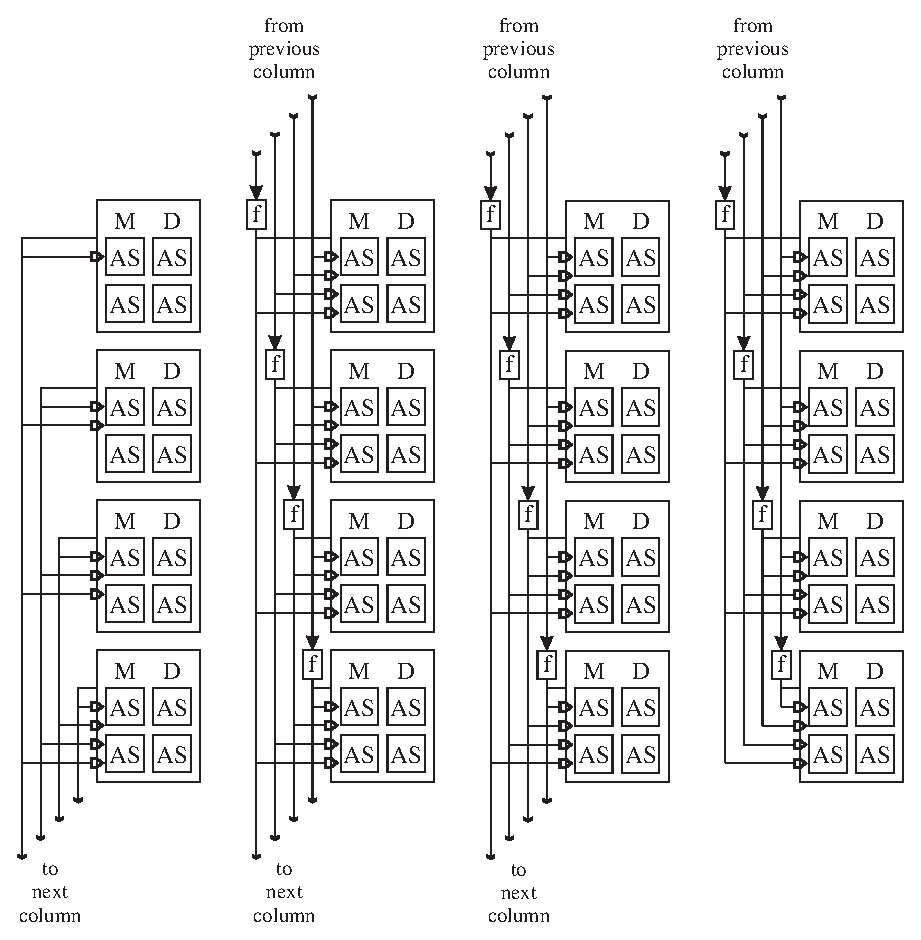
\epsfig{file=frwdbuss.eps,width=5.50in}
\caption{{\em Forwarding buses.} For this example a
sharing group size of 2 ML
instructions is assumed, as before,
along with an instruction window length of 32 instructions, folded to
8 rows by 4 columns. Forwarding spans are 8 instructions long. Blocks with
`f' in them are the forwarding registers. Note: this is the logical view.
With column renaming, all physical columns look the same as the middle
two columns here, with the buses from the last column wrapped around to
the first column.}
\label{forwardingbuses}
\end{figure}

Because instruction output results only
need to be forwarded for the lifetime of the ISA register in the
program, in our invention
results are only first forwarded a number of active stations
that roughly matches a typical register lifetime.  This forwarding
distance is termed the {\it forwarding span}.  Each active station
snoops all forwarding buses from the last span's-worth of active
stations to get the register inputs needed for its execution.
Each sharing group originates a forwarding bus that covers the
implementation's designated forwarding span.  For example, if an
instruction window consists of 256 ML active stations and these are
further divided into sharing groups containing eight active stations
from an ML column (and eight from a DEE column) then there would be 32
sharing groups each originating a forwarding bus.  If we assume a
forwarding span of 32 this means that at
any active station there would be $span-length/group-size = 32/8 = 4$
forwarding buses that would need
to be snooped by each source input.

In order to handle
those situations where an output result from an instruction is
needed in instructions located beyond the forwarding span of its
forwarding bus, there exists a register at the end of the bus (located
in the sharing group just after the last group snooping the bus).  This register is
termed the {\it forwarding register}; see Figure~\ref{shareforward}.
This register then contends
with the forwarding requests originating in its sharing group to
forward its result on that sharing group's forwarding bus.  The process
will result in output values being forwarded for the next forwarding
span number of active stations.  This forwarding process is repeated
across multiple spans and is stopped
when the forwarding
span of a result contains an active station having an output with
the same ISA register destination as the result.
The later instruction originating a
new value for that ISA register is now responsible for forwarding its
output value in the same manner.

\begin{figure}
\centering
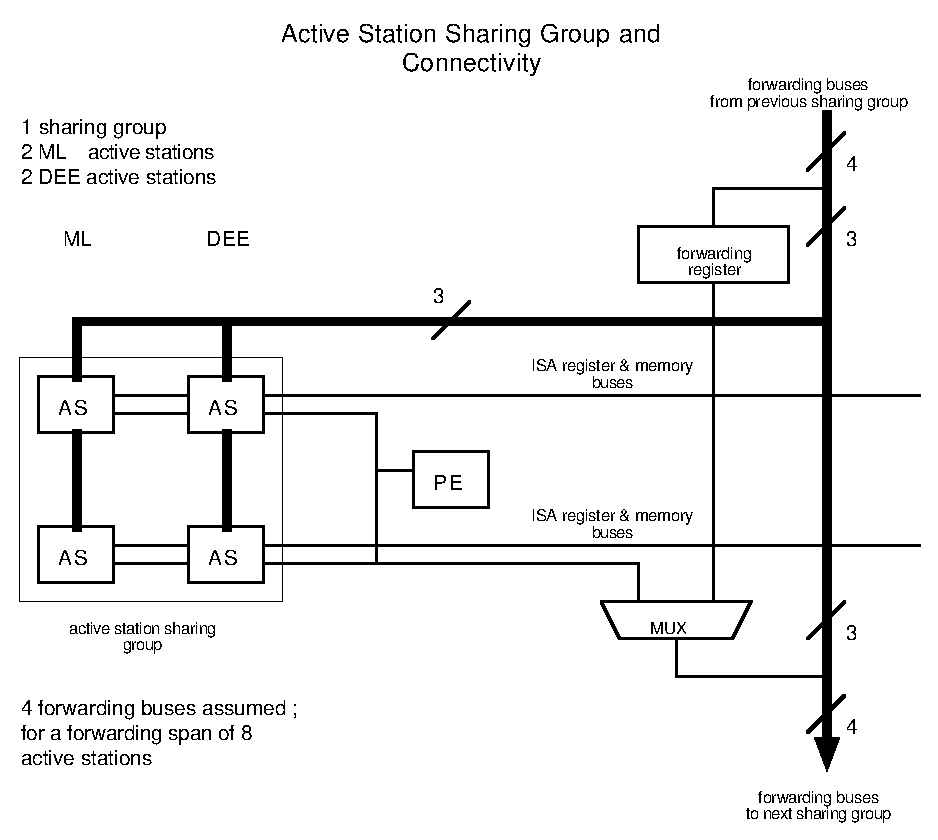
\epsfig{file=group.eps,width=4.50in}
\caption{{\em Sharing group forwarding structure.}
Each group has these components and connections to achieve
result forwarding beyond a forwarding span.}
\label{shareforward}
\end{figure}


Note that when instruction output results need to be forwarded to
stations beyond the implementation forwarding span there is at least
one clock cycle delay in the forwarding process due to the presence of
the forwarding register.  This register is minimally needed because of
possible contention for the forwarding bus of the sharing group the
forwarding register is associated with.  Note that more than one clock cycle
delay may
be incurred if the sharing group that is performing the forward also
needs to forward one of its results in the same clock cycle.  Delaying
a forward from a previous sharing group will not typically be a
performance problem since the need for a result created a long time in
the past is not as urgent as needing a result that was generated in the
more recent past of the program instruction stream.

\paragraph{Scalability: }
One of the key advantages of this invention is that it is the first
ILP machine
that is scalable, to our knowledge. By ``scalable'', we mean that the
hardware cost (amount of hardware) of the machine grows linearly with
the number of Processing
Elements. Machines with dependency matrices grow at least as quickly as
the square of the number of PE's. The hardware cost of existing machines
also typically grows with the square of the number of PE's.

The hardware cost of the resource flow machine grows no faster than
linearly because there is no dependency storage, generation or checking
hardware and because the size of the forwarding buses is fixed, that is,
the forwarding span normally stays the same regardless of the number
of PE's or active stations. Since the number of buses grows as a constant
fraction of the number of active stations, the hardware cost of the
buses also grows linearly with the number of PE's.

\paragraph{Absolute Hardware Cost: }
A preliminary spreadsheet analysis indicates that the invention will use
approximately 25 million transistors, including the 32 PE's. This is
under the typical limit quoted for designs of high-end microprocessors
getting underway in the near future: 100 million transistors. It is
also well under the 1 billion transistors often postulated as being
available on a chip in the not terribly distant future.

\paragraph{Logic Delay: }
This invention also has advantages over competing designs in its circuit
delays. Typically, a processor's performance is highly tied to the
operating frequency of its clock; the greater the frequency, the better
the performance. Thus, keeping the clock cycle time (equal to the inverse
of the clock frequency) low is paramount. One of the major objections to
building processors that exploit much ILP while determining the parallel
instructions in hardware (``brainiacs'') is that signals need to be
sent across much of the chip. As chips have increased their hardware
densities and as clock frequencies have increased, it takes more (multiple)
clock cycles for a signal to cross a chip. Therefore, any design that
requires global chip communication for all operations is at a large
disadvantage: the increase in ILP obtained will be at least partially
offset by a larger cycle time (reduced frequency) or a greater number
of cycles to perform a given amount of work.

The resource flow computer solves this problem by keeping most communication
among the active stations local. First, note that communication between
active stations should normally be completed in less than a cycle.
With the forwarding bus architecture of the invention,
most of the time a given active station will only communicate
with the number of active stations in a forwarding span, much smaller than
the total number of active stations. Further, it is likely that chip
layout optimizations can be performed to keep the total forwarding span
length of a single bus short, taking up a fraction of a dimension of a chip,
and thereby keeping the cycle time small.

\paragraph{Active Station Overview: }
The active station is based on the classic Tomasulo {\it reservation
station}, but has significantly more functionality. Like a reservation station,
the main function is to {\it snoop} or look at one or more buses carrying the
results of the computation from the processing elements, {\it snarfing} or
copying the information from a bus into the station's own storage. A reservation
station snarfs the data when the register address on a bus is equal to the contents of
one of the station's source address registers. In a reservation station the
corresponding instruction is fired (sent to a processing element) when all of its
sources have been snarfed.

Active stations differ in the following respects:
\begin{enumerate}
\item Time tags and ISA register addresses
are used instead of the arbitrary renaming addresses in the Tomasulo algorithm.
The Tomasulo
algorithm does not explicitly represent time in its reservation stations;
correct execution order is maintained by having computations chained to
follow the data flow of the code in the window. The resource flow computer's
use of time tags allows it to dynamically change the ordering of instructions
and when instructions get new data.

\item There are three more conditions for snarfing data for a total of four
conditions; for each source in the active station, the conditions are:
\begin{enumerate}
\item the broadcast register address must equal the source address (same
as before);

\item the broadcast register value must be different from the current
value of the source;

\item the broadcast time tag must be less than the time tag of the source (the
latter is equal to the time tag of the station);

\item and the broadcast time tag must be greater than or equal to the time tag of
the last datum snarfed for the source.
\end{enumerate}

The latter two conditions ensure that only the register value produced
closest to the active station, but not after it, is used by the source.

\item The active station uses a novel form of predication. The station
incorporates a small amount of logic to make predicate calculations.

\item Except for branching outside of the window, there are no traditional
branches held in active stations.

\item The predication mechanism works similarly to the snooping and snarfing
mechanism for data communication. Therefore there is a unified approach to
the handling of control flow and data flow.
\end{enumerate}

The operation of the resource flow computer is best understood by first
examining the detailed structure and rules of operation of an active station;
we do so now.


\subsubsection{Active Station Details}
Each instruction in the instruction window is held in an {\it active
station}; see Figure~\ref{activestation} for a structural view. We now describe the
contents of each active station including both storage registers and logic. For each
storage element we provide a description of the storage, its typical quantity and
size, and its abbreviation [NAME].
Each active station has the following contents:
\begin{enumerate}
\item One or more source input data registers. These are the traditional inputs to the
instruction, e.g., if the instruction is: {\tt r1 <- r2 op r3} these are {\tt r2}
and {\tt r3}.
Typically each is a 32-bit register.
[RIDAT]
\item For each input data register, an input data register address register. In the
example, the values held are: ``{\tt 2}'' and ``{\tt 3}''.
Typically each is an 8-bit register. [RIADDR]
\item One input data register with the same address as the destination data register;
in the above example the data value is {\tt r1in}, generated prior to
this instruction. Typically a 32-bit register. [ROIDAT]
\item One output or destination data register; in the above example this is {\tt r1}.
Typically a 32-bit register. [RODAT]
\item One address register for the output (and extra input) register, e.g., ``{\tt 1}''.
Typically an 8-bit register. [ROADDR]
\item For each input data register, a register containing an equivalent of the
time tag of the last datum snarfed. Typically each is a 39-bit register, one bit for
each earlier active station in a forwarding span snooped by this station
(total of 32 bits), and one bit for each prior forwarding span (total of 7 bits). [TTMASK]
\item One input predicate register. Typically a 1-bit register. [pin]
\item One input predicate address register. Typically a 9-bit register. [pinaddr]
\item One input cancelling predicate register. Typically a 1-bit register. [cpin]
\item One input cancelling predicate address register. Typically a 9-bit register.
[cpinaddr]
\item One output predicate register. Typically a 1-bit register. [pout]
\item One output cancelling predicate register. Typically a 1-bit register. [cpout]
\item A register holding the (possibly decoded) opcode of the instruction.
Size depends on realization; say it is typically a 32-bit register. [INSTR]
\item One instruction predicate; this is the value of the
predicate used by the instruction itself to enable the assigning of its normal
data output
to the output register. Note that this is not the same as pin or pout. Typically
a 1-bit register. [pI]
\item An instruction status register [SR] with the following status bits:
\begin{enumerate}
\item Instruction
Issued - indicates if the instruction has been sent to a PE for execution; this
is needed for multicycle instructions. [II]
\item Really Executed - indicates if the instruction has actually executed.
Optional. Will not be further discussed herein. [RE]
\item EXecuted - indicates if the instruction has executed. This bit is cleared if
a new datum or predicate or cancelling predicate is snarfed, forcing the instruction
to re-execute. [EX]
\item Branch Prediction - if the instruction is a branch, indicates the value of the
last prediction or execution of the branch; 1 -$>$ taken, 0 -$>$ not taken. [BV]
\item Address Valid - if a load or store memory reference instruction, indicates if the
memory address is valid (has been computed). Note that memory reference instructions
execute in two phases: address computation, using a PE, and the actual data load or
store via the memory system. [AV]

\end{enumerate}

\end{enumerate}

Note: explicit time tag registers are not needed for the predicate and cancelling
predicate since the time tag values are the same as the predicate address and
the cancelling predicate address. Also, it is not necessary to know the time tag
of the last predicate or cancelling predicate snarfed due to the predicate
chaining.

\begin{figure}
\centering
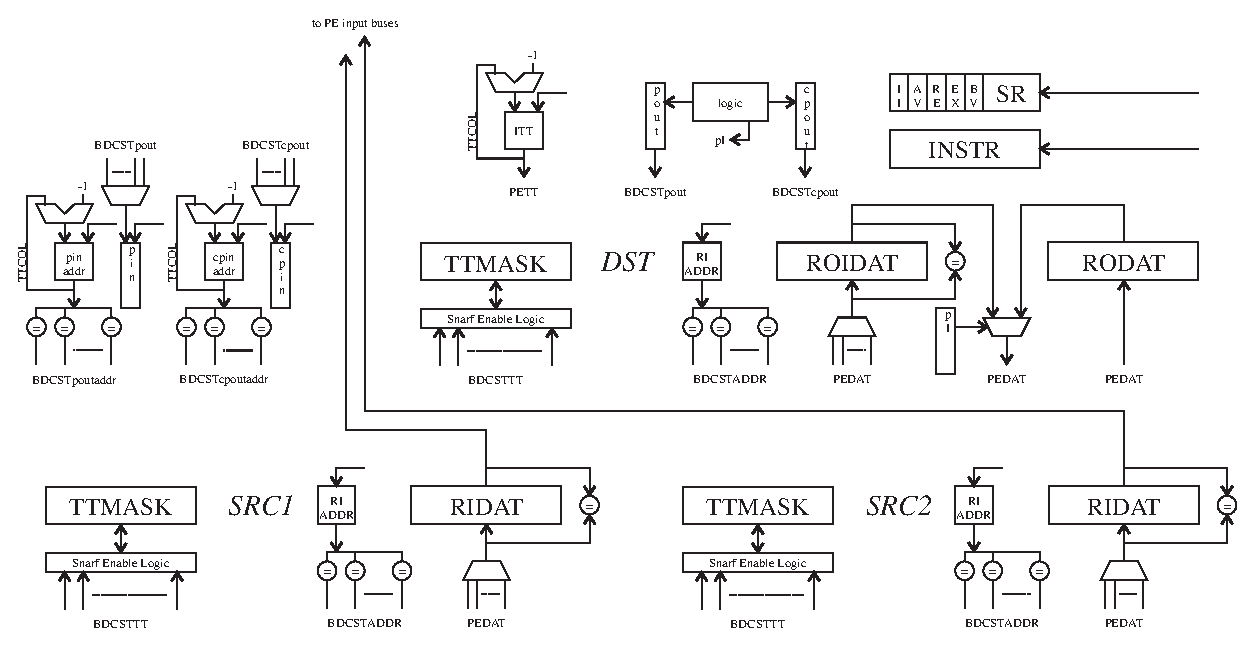
\epsfig{file=actstass.eps,width=6.50in}
\caption{{\em Active Station.} Each station has these components and connections to
the rest of the CPU.}
\label{activestation}
\end{figure}


Logic in or associated with each active station:
\begin{enumerate}
\item Column decrement logic - decrements the column part of time tags being
shifted from right to left in the instruction window. One decrementer for each time tag
or time tag derived address, i.e., 3x RLSTTT, pinaddr, and cpinaddr, for a total of five
3- or 4-bit decrementers.

\item Predicate and cancelling predicate computation logic - computes pi, pout and
cpout. Two AND gates and one OR gate.

\item For each data input register, an equality comparator determining whether the new
value of the input data differs from the old. Typically 32 exclusive-OR gates for
each of the three data inputs and combining AND-trees for each. 

\item For each data input, an equality comparator to determine if the data on a
broadcast bus has the same register address as the input. 
Typically 8 exclusive-OR gates and an AND-tree per comparator.
One per broadcast bus.

\item For each TTMASK register logic to detect whether a broadcasted datum is
closer in time to the station's time tag than previously snarfed data.
This is conservatively estimated to be less than 1,000 transistors.

\item Predicate matching comparators, one for pin and one for cpin - equality
compares (c)pinaddr with address of (cancelling) predicate on each (c)p broadcast bus.
Typically less than 
8 exclusive-OR gates and 1 AND-tree for each predicate and cancelling
predicate per (c)p broadcast bus. 

(c)pout are directly broadcast
from the active stations, bypassing the PE's.
Predicate bus congestion is alleviated by adding a bit
to each instruction indicating whether or not
its predicate outputs are needed - easily determined at instruction
load time with hidden-explicit
predicate-assignment hardware - and then only using a (c)p
broadcast bus from an active station if the predicate is needed.

\item Firing logic - takes the outputs of the comparators and determines if either
the data or predicate outputs should be computed and/or broadcast. Also computes
whether and which broadcast bus data or predicates should be latched into the
instruction's input registers. (pout and cpout
are always computed within an active station, due to the simplicity of the logic
needed.)

\end{enumerate}

The concept and details of an active station are novel. It is the most
important component of
the resource flow computer.

\subsubsection{Operation, Including Active Station Firing Rules}
The operation of the invention has similarities with existing
machines but also has some key differences.  This section will provide
a more detailed discussion of the dynamic operation of the machine as
it executes a program.  For the purposes of this discussion the initial
boot-up of the machine will be the starting point.  In other words, the
machine is currently empty of any loaded or executing instructions.
First an overview of the machine execution is given followed by a more
detailed description of what occurs within an active station.

In general, operation of the machine will proceed from
instruction-fetch, to branch target tracking, to instruction staging in
the station load buffer.  Next, the entire column of instructions in
the station load buffer is left shifted into the right-most column
of the active stations in the instruction window (reference
Figure~\ref{highlevelma}).
This is termed the {\it load} operation.  The
station load buffer is always the same length as a column in the
instruction window in order for this instruction load operation to
occur as a broadside left shift operation in one clock cycle.
These above operations
repeat until the entire instruction window is nominally loaded with
instructions through the left shift-like load operations.  Note that
the authors usually use the term {\it left-shift} for describing the
broadside instruction load operation but this operation can be
accomplished using a renaming scheme on the active station column
addresses in the instruction window. Recall that renaming allows a
physical column to function as any logical column; this is
transparent to the user.

Fetched instructions will also nominally be allocated cache lines in
the I-cache (if the corresponding memory page and physical hardware is
set to allow that).  This increases the effective instruction bandwidth
or maximum allowable rate of instruction fetch.
As instructions are fetched they are then
decoded.  This is, so far, similar to most all current machines.

Once the instructions are decoded, branch type instructions are
identified.  The target addresses of branch instructions are computed,
where possible, and an entry is made in the branch tracking buffer that
includes the time tag of where that branch instruction will be placed
in the instruction window when the branch is loaded.  The target of
the branch is also placed into the tracking buffer entry.  This
tracking buffer information is used to dynamically track the
instruction domains of instructions within the instruction window.
(See the accompanying invention disclosure on ``...Predication...''
by the same authors for more information on the branching hardware.)

Instructions are then put into the active station load buffer.
The station load buffer serves as a staging area to accumulate
instructions until they can enter the instruction window.  When the
instruction load buffer is full, and the leftmost column contains nothing
but fully-executed instructions (able to be retired), an operation
analogous to a left shift occurs amongst all of the active station
columns and those instructions currently staged in the station load
buffer.  Source register values for the
loading instructions are taken from the
architected register files (one per instruction window row) at the time
the load occurs.

Once instructions are loaded into an active station, they are allowed
to compete for execution, main memory, and architected register
file resources.  Instructions compete for execution resources
within their sharing groups.  When an instruction sends information to
an execution unit for processing, this is termed {\it instruction
issue}.  Unlike conventional machines, an instruction can be issued to
execution or function units many times during the time that
the instruction is in
the instruction window.  This will be discussed in more detail later.

Instructions compete for memory bandwidth with all of the other active
stations in the other instruction window columns located in the same
row.  This is illustrated with the contention for the horizontal row
buses to the memory interface buffers shown in Figure~\ref{memory}.

Active
stations also compete to store their output register results into
a row's
architected register file copy with all other active stations on the same
instruction window row.  This is illustrated with the contention for
the horizontal row buses to the ISA register files shown in
Figure~\ref{isaregisters}.

Speculative reads to main memory are allowed at any time during an
instruction's execution but memory writes are only allowed, in the
current implementation, at instruction retirement time.
When the instructions in the
left-most column of the instruction window, those with the smallest
time tags, have all completed executing, they are ready for
retirement.  Retirement may occur immediately, independently of
instruction window loading.

Therefore, in
general, instructions can be thought of as proceeding through fetch,
decode, branch tracking, staging, load, issue, and
retirement/write-back stages. We know give more detailed explanations
of the functioning of the resource flow computer's components.

As noted already, an instruction in an active station can be issued to
an execution unit more than once.  An instruction is issued to an execution
unit when one of its inputs is changed but which has a time tag
later than or equal to that of the last source value
that was acquired by the instruction's input.

An
active station snoops all forwarding buses originating from earlier
sharing groups for changed input values.  As discussed earlier,
values from stations more than a forwarding span earlier go through
one or more forwarding registers; logically, we look at the buses as
being uniform and going all the way back to the earliest station in the
window.

Values are forwarded on these
buses with the address of the architected register that is being
changed along with its value, and with information indicating its
time tag (time order) within the instruction window.  All forwarding
buses are snooped by an active station for updates corresponding to
those registers that are the station's inputs.
The register address comparisons
are done using the RIADDR registers and comparators associated with the
two register sources and register destination of the active station.

Forwarded branch predicates (representing control flow dependencies)
and forwarded output data values are snooped and processed somewhat
differently.  Considering data values first,
the physical arrangement of the data forwarding
buses originating from the sharing groups ensures that
only values originating from
previous instructions are considered as possible inputs.  However, a
means must be used to ignore values coming from previous instructions that
are earlier in time than a previously snarfed data value.  This is
accomplished by using the time tag mask registers (TTMASK) in the
active stations.  Again, there is a time tag mask associated with all
data oriented sources in the active station (including the relay source
value for the instruction's output if there is one).

The time tag mask is actually physically two masks, one representing
the last forwarding span (32 assumed for this discussion) of active
stations and is termed the {\it forwarding bus time tag mask}.  The
other mask represents each of the previous forwarding spans (normally a
column's worth of active stations) and is termed the {\it forwarding
column time tag mask}.  The forwarding bus time tag mask in this
example is 32 bits wide, one bit for each of the 32 active stations
being snooped by the active station.  The column mask in this
implementation example is seven bits wide, each bit representing one
of the previous seven forwarding spans (there are eight forwarding
spans in the implementation being described).  Both the forwarding bus
time tag mask and the column time tag mask are ordered corresponding to
the time order of the forwarding buses and previous columns
respectively.  As a convention, we assume that both masks are ordered
such that the right-most bits correspond to active stations (in the
case of the forwarding bus time tag mask) and forwarding span columns
(in the case of the column time tag mask) are from active stations
earlier in time.  Bits which are set in the masks represent forwarding
buses or forwarding spans that are allowed to be snarfed by this active
station.  Bits which are cleared serve to prevent the snarfing of
data.

If a source input is snarfed from the last forwarding span number of
active stations (within the last 32 active stations in this
implementation), then the position of the bus, as ordered corresponding
to the time of the active station that is originating data on it, is
compared with the forwarding bus time time mask.  If the corresponding
bit in the time tag mask is clear, then no snarfing is performed.  If
the bit in the time tag mask is set, then the data value is snarfed and
all bits to the right of the bit just examined (earlier in time) are
cleared.  The same sort of operation is done analogously with the
column time tag mask when a forwarded value originated from an active
station prior to the preceding forwarding span number of active
stations.  Within each forwarding span of active stations, a generated
output value will never be forwarded beyond a forwarding span (32) if
some instruction within the next 32 active stations also outputs a
value to the same ISA register address.  Since only one output data
value per register address
will ever be forwarded beyond a forwarding span of active
stations, this scheme of using a column mask and a forwarding bus mask
ensures that only a value equal to or later in time than that indicated
by the mask (but earlier than
the time tag of the snarfing active station) will ever be snarfed.
Additionally, a data output is only snarfed if the actual value of the
data has changed from the previously snarfed or held value.  This
latter comparison is done with the equivalence comparators shown in
Figure~\ref{activestation} located along with the RIDAT and ROIDAT
registers.

Predicates are snooped and snarfed in a similar manner as data values,
but since predicates are chained with a hardware oriented linked-list
scheme and every predicate address is unique to its generating station,
there is no need for the time restriction scheme associated
with snarfing of data values.  Only the predicate addresses being
snooped need be compared, just as register addresses were compared with the
forwarded output data snooping.

As previously mentioned, predicates use a separate forwarding bus
structure from the data forwarding buses and their operation differs,
but the block diagram is the same (see Figure~\ref{forwardingbuses}).
The predicate buses are only one bit wide. There are two identical
sets of buses, one
for the regular predicates and one for the cancelling predicates.
As with data the predicate value and its address are broadcast on a bus
by a sharing group. The predicate may go through multiple forwarding
registers before being superseded. With predicates, {\underline any}
later predicate being broadcast, that is having any other predicate
address, terminates the broadcast of all earlier predicates. This
is due to the predicate chaining being done with active stations.

It is possible that the ideal sharing group size for predicates may be
different than that for data. This is allowable by the invention.
The predicate system is basically independent of the data system,
although it may be convenient to make their dimensions the same.

Note that predicate register addresses are actually the
time tags of instructions generating the specific predicate.
For this reason, there must exist
arithmetic decrementing logic needed to subtract one from the
column address part of the time tag when a logic left-shift
operation occurs on the instruction window.

As with register values and data dependencies, predicates are chained to
form control dependency trees corresponding to those
in the program being executed.
Just as when a new updated value of a data source becomes
available for an instruction, causing it to become enabled to
execute again, so too can a changed predicate value cause
an instruction to enable another execution.  A predicate
value for an instruction can change when a previous branch,
on which the instruction is control dependent, either becomes
resolved mispredicted or changes its prediction for some reason.

If a predicate value is broadcast but its value does not change, any
instructions depending on that predicate rebroadcast their output
values.  This requirement handles the situation where a branch
prediction was changed causing a replacement of a segment of the ML
path with a corresponding DEE path.  In this case, the output values of
those instructions beyond the branch having the prediction that changed
have to be rebroadcast. This is because the DEE output values
are usually different than the output
values that were last broadcast from the former ML path of active
stations.  Schemes to selectively avoid this later re-broadcasting of
output values are being considered. However, this would be to tune
the machine's performance; the present scheme has the necessary
functionality and does affect the operation of other parts of the
machine.

In those cases where an instruction is simultaneously the target of two
or more branches, extra active stations are allocated for the
instruction at instruction load time in order to utilize the extra
cancelling predicate register hardware in the active station.
Figure~\ref{activestation} showed only one set of cancelling predicate
hardware but an implementation may contain more than one set of this
hardware as an optimization.  One set of cancelling predicate hardware
is required for each branch that an instruction may be the target for.
In cases where an instruction is the target of more than one branch and
where there are not enough cancelling predicate hardware sets in the
active station to accommodate the number, the cancelling predicate
hardware sets of the following active station is also used for
detecting when a predicate changes.  In any event, an instruction is
enabled for re-execution when any of its input predicates or cancelling
predicates changed or are just rebroadcast.

Finally, it has been shown that instructions can be speculatively
executed far ahead of the committed execution state while still
being able to eventually re-execute as necessary in order to
eventually correspond to the final committed state.
We have created mechanisms that manage both the data dependencies and
the control dependencies that trigger an instruction to re-execute
when either an input predicted data value changes or an input
predicated
control condition changes.  Using these means, instructions
can be dispatched for execution according to a priority scheme
that only has to consider the availability of resources
in the machine.  Hence, this new execution model has been termed
resource flow execution.

\subsubsection{Examples of Operation}
Some simple examples of code execution in the resource flow machine
will be 
given in this section in order to illustrate the snooping/snarfing
operation across active stations. We first give examples illustrating
the data transmittal features of the invention. Examples incorporating
predication follow that section.

\paragraph{Data Examples: }
A snippet of code that we will consider for the first two examples
follows. We will assume that each of the
instructions are loaded into active stations with the same row designation
as the instruction number. We also assume that each instruction is in
a different sharing group, so the instructions do not compete with
each other for a PE.

\begin{verbatim}

00	r9 <- r0 op r1
10	r3 <- r5 op r6
20	r3 <- r7 op r8
30	r2 <- r3 op r8

\end{verbatim}

\subparagraph{Data Example 1: }
In the first example we will look at how instruction number 30 gets the
correct value for one of its sources, namely register
{\tt r3}. Refer to Figure~\ref{ex1} for an illustration of the execution
timing.

\begin{figure}
\centering
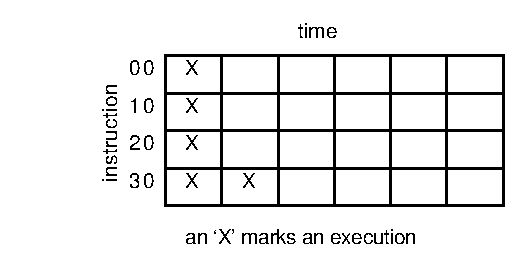
\epsfig{file=e1.eps,height=1.50in}
\caption{{\em Timing of the code example, scenario 1.}
In this example all of the instructions are able to execute in
the first cycle. Execution of an instruction at a given time is
indicated by an `X'.}
\label{ex1}
\end{figure}

Instruction number 00 does not produce
any outputs used in the next few instructions that
we will consider so there is no data dependency and its output 
is never snarfed by the later instructions.
The execution of instruction 00 therefore
does not further impact the correct operation of instruction 30.

At load time, instruction 30 will
load register
{\tt r3}
from the ISA register file as an initial value guess.  
This may not be
the correct value that instruction 30 should be using but 
we use it anyway as a predicted value.
In this example, instructions numbered 10 and 20 both generate
an output to register 
{\tt r3}.
Instruction 30 will snoop the buses looking for a broadcast of
{\tt r3}, and will only snarf it if the broadcast value differs from
the current value of {\tt r3} held in instruction 30's active
station.
That station will watch for the address
of that register (the number {\tt 3} in this example) to
appear on one of the four data output forwarding buses the station is
connected to (following Figure~\ref{forwardingbuses}).

The instructions may all execute immediately after they are loaded,
assuming their corresponding PE is free.  Let's assume that this happens
and all instructions execute in the same clock immediately upon being
loaded.
Instruction 30 will now have a result based on what register
{\tt r3}
was at load time but a new output for this
register has just been produced by both instructions 10 and 20.
Instructions 10 and 20 will both broadcast forward their new output
values for
{\tt r3}
on separate forwarding buses; instruction
30 is snooping for a new update
to register
{\tt r3}
on both of these buses (and the others).

Updates coming from both instructions
10 and 20 will be considered for snarfing by instruction 30 since
its forwarding bus time tag mask initially has all bits set.
Instruction 30
will see that the output from instruction 20 is later
in time than that from instruction 10, so it will snarf instruction
20's value
and update its forwarding bus time tag mask by clearing all bits
to the right (earlier in time) than the bit corresponding to
instruction 20 above.  No register updates from instruction 10
will ever again be snarfed by instruction 30.  New updates
from instruction 20 will still be considered though since its
bit in the forwarding bus time tag mask is still set.

\subparagraph{Data Example 2: }
Another example, still referencing the code snippet above
in Data Example 1,
is that upon the instructions all being loaded in the same
clock period, only instructions 00 and 10 can execute immediately.
(Instructions 20 and 30 may not be able to execute due to
other instructions, not shown, having priority for execution
resources.)
Again, we focus on what instruction 30 does to get a correct
value for register
{\tt r3}. See Figure~\ref{ex2} for the code execution timing.

\begin{figure}
\centering
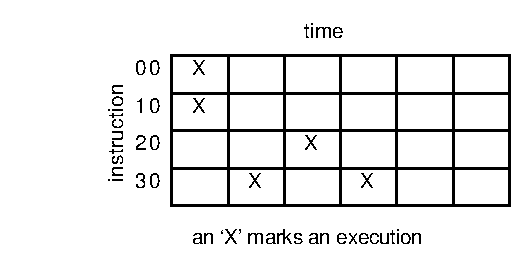
\epsfig{file=e2.eps,height=1.50in}
\caption{{\em Timing of the code example, scenario 2.}
In this example instructions 20 and 30 are not able to execute
immediately. Execution of an instruction at a given time is
indicated by an `X', as before.}
\label{ex2}
\end{figure}

After being executed, instruction 10 will broadcast 
its updated value for register
{\tt r3}
on a forwarding bus.
This value will be snarfed by instruction 30 since all of its
time tag mask bits are still set.  Upon snarfing the updated
value from instruction 10, all time tag bits to the right of
it will be cleared to zero.  In our current example, there
were no instructions earlier than instruction 10 within the instruction
window which generated an output to register
{\tt r3}
but the bits are cleared just the same.

Instruction 30 will now execute using the updated register value.
Also, if it had already executed, the act of snarfing a value will
enable the instruction to execute again.  Of course, the newly broadcast
value would not have been snarfed if its value did not change, nor would
instruction 30 have executed.

Finally, instruction 20 gets a chance to execute and afterwards it
broadcasts its output value on a forwarding broadcast bus, as always.
Since instruction 20 is later in time than instruction 10,
the bit in the time tag mask of instruction 30 which corresponds
to instruction 20 will still be set indicating that a snarf
is still possible from that instruction.

Note that if instruction 20 had executed before instruction 10,
instruction 30 would have cleared the enabling time tag bit
corresponding to instruction 10, so that once instruction 10
did execute, its value would be ignored by instruction 30. This
is exactly what is desired: an instruction should use the input
value from the closest but earlier instruction for the final
value of the input.

>From a performance point of view, the above examples illustrate that
an instruction will execute as soon as it possibly can. Further,
if the data value prediction was correct, or the instruction's
inputs do not
change even if they have been re-evaluated, then the instruction
need not execute or re-execute, resp. Therefore the performance of
this invention is potentially much greater than competing techniques.

\subparagraph{Data Example 3: }
Now consider the simple code excerpt below, with the execution timing
as shown in Figure~\ref{ex3}.

\begin{verbatim}

00	r3 <- r5 op r6
10	r1 <- r3 op r1
20	r3 <- r5 op r6

\end{verbatim}

\begin{figure}
\centering
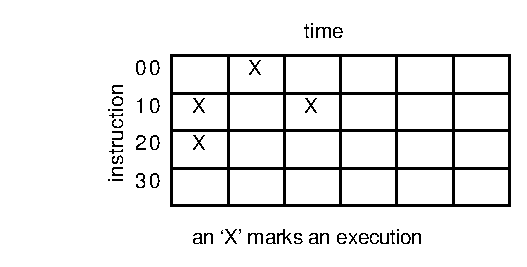
\epsfig{file=e3.eps,height=1.50in}
\caption{{\em Timing of the code example, scenario 3.}
In this example instruction 10 does not re-execute due to an update
of its input register from instructions 10 and 20 but does
finally re-execute after an update from instruction 00.
Execution of an instruction at a given time is
again indicated by an `X'.}
\label{ex3}
\end{figure}

In this example we assume that instructions 10 and 20 get to execute
before instruction 00 does.  We will also assume that instructions
10 and 20 both execute in the same clock cycle.
Initially, as always, the sources for these instructions
are taken from the ISA register file at load time.

Firstly, it should be noted that after instruction 10
executes at least once, it will not necessarily be enabled to execute
again even though one of its input sources has changed, namely
register
{\tt r1}.
It is not enabled to execute again for this input source change because
the new value of
{\tt r1}
that is generated is only forwarded to instructions {\it later}
in time order than instruction 10.  
Instruction 10 will never, therefore, see register
{\tt r1}
being updated due to its own broadcast of that register.

In like manner, instruction
10 will not be enabled to execute simply because of the register change
of
{\it r3}
from instruction 20.  The output from instruction 20 will
only be broadcast forward to later active stations and
the active station holding instruction 10 is not snooping for it.

Finally, when instruction 00 does get to execute, it will
forward broadcast an updated value for register
{\it r3}.
Since instruction 10 is snooping on changes to this value,
it will be enabled to execute again and will eventually do so.

\subparagraph{Data Example 4: }
Finally with regard to data dependencies alone, we consider
the following code excerpt.

\begin{verbatim}

00	r2 <- r0 op r1
10	r3 <- r2 op r0
20	r2 <- r0 op r4
30	r5 <- r2 op r4

\end{verbatim}

The time order of the code's execution is shown in
Figure~\ref{ex4}.

\begin{figure}
\centering
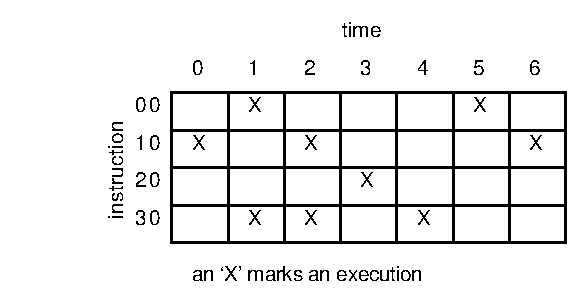
\epsfig{file=e4.eps,height=1.50in}
\caption{{\em Timing of the code example, scenario 4.}
In this example an output data broadcast from instruction 00
in time cycle 4 enables one later instruction to
execute but not one later still in the program order.
Execution of an instruction at a given time is
again indicated by an `X'.}
\label{ex4}
\end{figure}

In this example we will put together some of the
code execution and data dependency rules already illustrated
separately.
We assume that after all of the above instructions are loaded
that instruction 10 gets to execute first.
Next, instructions 00 and 30 get to execute together in a single
clock.  Instruction 00 then broadcasts an update for register
{\tt r2}.
This enables or re-enables instructions 10 and 30 to execute again.
They do so in the next clock cycle.  Next, instruction 20 finally
gets a chance to execute.  Again an update for register
{\tt r2}
is broadcast forward.  This enables instruction 30 to execute again
but not instruction 10.
Finally, instruction 00 executes again for some reason.
Again, an update for register
{\tt r2}
is broadcast forward.  However, this update does not enable
instruction 30 to execute again since it had previously used
a value from instruction 20.  At the same time, this broadcast does
enable instruction 10 to execute again and it does so in the following
clock cycle.


\subparagraph{Data Example 5: }
Finally, this last data dependency example shows the
penalty incurred due to the finite forwarding span
in an implementation.  We will assume a forwarding span
of 32 for this example.  Consider the following
code excerpt.  Note carefully the distance that each instruction
is from each other.  This distance will interact with
the finite forwarding span to create extra bubbles in
the execution of instructions even though there may be no other
constraint preventing execution from occurring earlier.

\begin{verbatim}

000	r2 <- r1 op r0
040	r3 <- r2 op r0
080	r4 <- r2 op r0
120	r5 <- r3 op r0

\end{verbatim}

The execution sequencing of this example is shown in
Figure~\ref{ex5}.

\begin{figure}
\centering
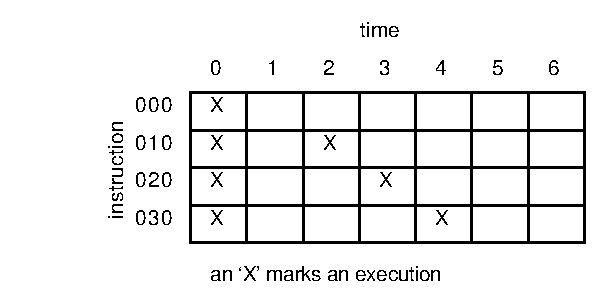
\epsfig{file=e5.eps,height=1.50in}
\caption{{\em Timing of the code example, scenario 5.}
In this example an output data broadcast is shown being
delayed by the processing of being forwarding
to a following forwarding span through the use
of the forwarding register.
Execution of an instruction at a given time is
again indicated by an `X'.}
\label{ex5}
\end{figure}

All instructions are loaded and we assume that all
instructions execute immediately and complete in one clock cycle.
Further, we assume that any of these instructions are free
from execution resource constraints to execute in any clock cycle.
The output generated from instruction 000 to register
{\tt r2}
will be broadcast on a forwarding bus and its value will be snooped
by all later instructions.  Since there is no instruction
between instruction 000 and instruction 040 that uses 
register
{\tt r2} as an input,
that output forwarding broadcast operation will result
in the output broadcast being registered in the forwarding register
located at the end of its initial forwarding span.  This
is logically at the end of active station 31 or the start of active station
32
(they are numbered starting at 0).
The output of the forwarding register will then be broadcast
on the next forwarding span but has incurred a clock cycle delay.
This delay prevents instruction 040 from re-executing immediately
in cycle 1 and instead can only execute again in clock cycle 2
at the earliest.  The output broadcast from instruction 000
will again be registered in the forwarding register located
at the end of the second forwarding span (logically at the
end of active station 63).  This further causes instruction 080
which was also snooping for updates to register
{\tt r2}
to become enabled to re-execute.  We assume that it does so
at the earliest possible time which would be in clock cycle 3.
Finally, instruction 120 was snooping for updates to register
{\tt r3}.
An update to that register occurred in clock cycle 2 but because
instruction 120 is more than a forwarding span away from instruction
080, a forwarding register delay is again incurred before the update
is seen by instruction 120.  Finally, instruction 120 can execute
again at the earliest in clock cycle 4.

\paragraph{Predication Examples: }
Now some examples involving control dependencies are
examined. 

\subparagraph{Predication Example 1: }
Consider the following code sequence.

\begin{verbatim}

00	r2 <- r1 op r0
10	b_op r2, 030
20	r3 <- r1 op r0
30	r4 <- r1 op r0

\end{verbatim}

This example illustrates a simple minimal control dependency
situation.
Instruction 30 does not depend, either through a data flow dependency
of a control flow dependency on any of the instructions that
are shown to be before it.  The branch instruction 10 is data
dependent on instruction 00 (through register
{\tt r2}.
Instruction 20 is control
dependent on instruction 10 (the branch).
The execution sequence of this example is shown
in Figure
Figure~\ref{pex1}.

\begin{figure}
\centering
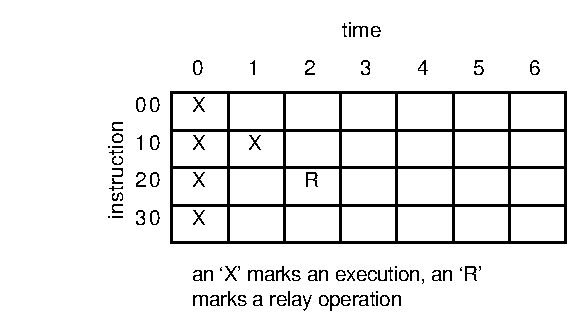
\epsfig{file=pex1.eps,height=1.50in}
\caption{{\em Timing of the code example, predication scenario 1.}
This example illustrates the exploitation of basic minimal control
dependencies, a significant contribution to
achieving higher ILP by taking advantage of independent
instructions beyond the joins of branches.
Execution of an instruction at a given time is
again indicated by an `X'.}
\label{pex1}
\end{figure}


We start by assuming that all instructions execute in a single clock
cycle and that they all execute immediately upon being loaded.
It is assumed that the initial execution of the branch in
instruction 10 (at time 0) did not change its predicate output.
However, since instruction 00 executed in clock cycle 0, we will
assume that its output value changed from what was originally loaded
at instruction load time.  Instruction 00 will broadcast forward
its new updated output (register
{\tt r2}).
Since instruction 10 (the branch) is data dependent on
register
{\tt r2}
from instruction 00, it will snoop for that update
and snarf the new value.  This will enable it to re-execute.
We assume that it executes at the earliest possible time.
This would be clock cycle 1.  On this execution, its output predicate,
essentially its branch prediction, does change.  The branch may either
have been resolved at this point or simply have made a new prediction
based on a possibly still speculative value of register
{\tt r2}.
Either case is handled the same.
A change in the branch condition will change its
predication output and this will be
broadcast out.
Instruction 20, being control dependent on the branch, will be snooping
for this predicate change and seeing that it has changed
will either become enabled for re-execution or re-broadcast
its relay output value.  Which is done depends on the original
value of the branch prediction; the new action will be the opposite
of the original action taken on the original prediction.
It is assumed that instruction 20 re-executes and it does so
in clock cycle 2.

In spite of the branch being predicted one way and then changed
to the other (whether re-predicted or resolved), it should be
noted that instruction 30 was not required to be re-executed as
a result.  This illustrates a basic minimal control dependency
which serves to facilitate higher instruction level parallelism (ILP)
by taking advantage of independent instructions located beyond the
joins of branch domains.


\subsubsection{Prior Work and Alternate Solutions}
\label{priorwork}
\paragraph{Comparison to Traditional Systems: }
See Section~\ref{background}.

\paragraph{Prior Work: }
Time tags have been used in two prior machines, to our knowledge.
Neither machine was built.

The first machine was the Metaflow processor\cite{Popescu91}.
Metaflow used time tags for a branch misprediction mechanism.
When a branch mispredicted, all instructions with tags
later in time than the branch's were squashed. This made it
easy to determine anywhere in the machine if an instruction need
to be squashed. This idea is only slightly related to our
use of time tags; our method is much more general and is applied
to data as well. Further, our mechanism is used to actually get the
right data to an instruction, something not attempted in
the Metaflow architecture.

The second machine is the Warp Engine
\cite{Cleary95}, based on the ``Time Warp''
concept of \cite{Jefferson85}, itself
being originally
devised for simulation. The Warp Engine uses ``timestamps'' in
a similar fashion to Metaflow. It goes beyond Metaflow by
executing some code or ``events'' speculatively, then rolling
back the state when necessary using ``anti-messages''. Some
code can be executed without regard to data dependencies, like
our invention, but data dependencies must still be computed and
maintained in order to determine to what point a state
rollback should go. The method used also requires the global
broadcast of a Global Virtual Time. This may have an effect on
the machine's cycle time. It also highly complicates the execution
algorithm. Lastly, the machine is able to make some memory
references speculatively, then re-execute the reference instructions
as necessary. In our invention both memory and register operations
are made speculatively within the processor, but the external memory
always contains correct state.

The closest thing to the invention's forwarding bus scheme is the
register reservation masking scheme used in the Multiscalar
Processor\cite{Sohi95}. Masking registers use a bit to indicate if
a register value generated in a prior task is needed by the mask's
(later) task. The bit is cleared once the value is transmitted.
It is not clear how values generated within loops are handled,
and the masks regenerated.
This scheme is quite different from our invention. Also, in Multiscalar
the register value production and consumption among code regions
(their ``tasks'', our ``forwarding spans'') must be determined by
the compiler and transmitted to the processor with the code for
execution. Hence, there is a code compatibility problem with
Multiscalar; programs must be re-compiled before they could be used
on the machine. However, this is usually impossible with commercial
code. Further, the multiscalar scheme is fully static, it cannot adapt
to changes in the contents of the instruction window as small or
large as can be handled in our invention.

Data value speculation has been used elsewhere, as discussed earlier.
It is likely that other specific methods of data value speculation
than ours could be advantageously incorporated into the invention.

The prior work of the lead inventor has already been cited and discussed.
This invention is a dramatic improvement on that work.

There is no other substantially relevant work to our invention, to
our knowledge.


%\subsubsection*{References}
\bibliographystyle{ieeetr}
\bibliography{cdgnew,cvrefs}



\subsection{Is this a new invention, different enough from any other invention,
including any that you may have previously disclosed, that it will carry new
claims?}
Yes. 

\subsection{What is the invention?}
It is a combination of: a new process, a new device, one or more new
products, and a new use for or
an improvement to an existing product or process.

\subsection{What are the immediate and/or future applications of the invention?}
Improving the performance of computers.
Near- and long-term application. Could start to use this in new designs today.

\subsection{Why is the invention better -- more advantageous -- than present technology?}
It allows substantially more speculation than prior techniques. It incorporates
Disjoint Eager Execution and Minimal Control Dependencies. These should give the
invention a high level of performance.

Also, the invention greatly simplifies and reduces the hardware needed to realize
Disjoint Eager Execution and Minimal Control Dependencies. Further, the invention
is scalable: its cost grows linearly with an increasing number of execution
units.

\subsection{What are its novel and unusual features?}
The concept of ``resource flow'' and ``squash flow'' are completely novel.
The time tag method of enforcing data and control flow is almost completely
novel. The process of only firing or re-firing an instruction only when an input
of the instruction has actually \underline{changed} is novel. The use of
the specific predication method is novel, and is itself the subject of a
companion disclosure. The uniform treatment of data and control flow is
novel.

\subsection{What problems does it solve?}
The eternal quest for more performance, preferably at little cost.

\subsection{How does the invention differ from present technology?}
See Section~\ref{background}.

\subsection{What problems does it solve or what advantage does it possess?}
See above.

\subsection{Is work on the invention continuing?}
Yes. It is being realized as the microarchitecture of a research machine called Levo.
A revised version of the Levo simulator is under construction at Northeastern
University, under my direction. We eventually plan to build a Levo prototype.

\subsection{Are there limitations to overcome or other tasks to be done prior to
practical application?}
The simulations must be done both to verify functionality, to determine the machine's
performance and to select good values for the machine's parameters, or ``dimensions'',
such as number of active stations to use.

\subsection{Are there any test data?}
The data from \cite{Uht95} indicate that we may obtain ILP on the order of 20-30
with DEE and Minimal Control Dependencies,
at least. The invention is better than the version of the machine studied earlier.

\subsection{Have products, apparatus or compositions, etc., actually been made and tested?}
No.

\subsection{What disadvantages or limitations does the invention possess?
Can they be overcome? How?}
The invention uses more hardware than original processors
but not a substantially larger amount, especially
given current hardware density trends (the number of transistors on a chip doubles
avery 18 months - Moore's Law). 

\subsection{Background: What is the field or art to which the invention applies?}
Computer central processing unit design.

\subsection{Does....earlier dated record of invention exist? Describe.}
Yes. In loose papers and my research notebooks, which I carry with me.
The invention was created
over a period of time, beginning on June 30, 1998 and ongoing, with the major
parts of
the invention created between June 17, 1999 and January, 2000. Some of
the corresponding
notebook entries and loose papers have been countersigned. I have included
copies of the main sections.

\subsection{What do you see as the commercial value of your invention?}
Potentially large, since it is applicable to all computer instruction sets.

\subsection{What firms may be, or are interested, and why?}
I have not approached anyone about this invention. A list of all
existing computer
companies would form the firms potentially interested in the invention,
in particular those
focusing on high performance. This would be to improve their product lines
and make them more competitive.

Example firms: AMD, IBM, Intel, Hewlett-Packard, ..... AMD
might be very interested,
because they are keen to gain more market share from Intel. Intel tends to be
an NIH company (Not Invented Here), but not absolutely.

\newpage

\section{Publications, Public Use and Sale}
\subsection{Has invention been disclosed in an abstract, paper, talk, news story, or
a thesis?}
Slightly. The lead inventor
described the big picture of the design in a talk on November 19, 1999
to the research group of Prof.\ Kaeli, one of the other inventors. It was a closed
meeting, all materials were marked confidential and the participants were asked
to keep the information confidential. Since this is the group that is helping
to design, develop and study the invention, this should not be counted as
a public disclosure.

\subsection{Is a publication or other disclosure planned in the next six months?}
Yes, one or more.

We plan on submitting one or more papers in early April, 2000 to two conferences taking
place in the Fall, and/or to submit a paper in June, 2000 to the International
Symposium on
Microarchitecture, taking place in November, 2000.

\subsection{Has there been any public use or sale of products embodying the invention?}
No.

\subsection{Are you aware of related developments by others?} Yes. See above.

\newpage

\section{Sponsorship}
WAS THIS RESEARCH SPONSORED?	YES.

\subsection{Government Agency: Yes}
This research was sponsored by the National Science Foundation under grants
MIP-9708183, EIA-9729839 and DUE-9751215. I am the Principal Investigator for
all of these grants.

\subsection{URI:} No. Northeastern???

\subsection{URI Foundation:} No.

\subsection{Private Industry:} No.

\subsection{Has the invention been disclosed to industry representatives?} No.

\newpage

\section{For Our Records}

\subsection{Names and titles of inventors:}

\begin{verbatim}
Associate Professor Augustus K. Uht, URI, lead inventor

Signature:

Date:



Research Assistant David Morano, Northeastern University, inventor

Signature:

Date:



Associate Professor David Kaeli, Northeastern University, inventor

Signature:

Date:



\end{verbatim}

\subsection{Contact for more data:} Augustus K. Uht, x4-5431, uht@ele.uri.edu

\subsection{Mailing Address for lead inventor:}

\begin{verbatim}
Augustus K. Uht
44 Torrey Rd.
Cumberland, RI 02864-1220
\end{verbatim}

\subsection{Name and title of institutional representative:}

\begin{verbatim}

Signature:

Date:

Quentin C. Turtle, Director
Industrial Research and Technology Transfer

The Research Office
University of Rhode Island
70 Lower College Road, Suite 2
Kingston, RI 02881

Tel.   (401) 874-2304
FAX    (401) 792-9089
\end{verbatim}

\end{document}

